\chapter{Intelligence artificielle}
\label{chap:chapter_3}
\section{Informatique et dermatologie}
L’informatique est une ressource omniprésente dans de nombreux domaines d’application. Sa faculté à nous divertir ou encore à nous guider dans nos choix quotidiens personnels et professionnels en fait un précieux allié. Sur un plan purement professionnel, ses atouts en comparaison à l’être humain peuvent se résumer à :
\begin{itemize}
    \item Sa rapidité à effectuer des traitements, parfois répétitifs, dans un temps réduit conjoint à l’évolution matérielle
	\item Sa robustesse face à l’erreur, sur des cas multiples
	\item Son objectivité face aux situations rencontrées.
\end{itemize}
De nouvelles pratiques font leurs apparitions, intégrant la machine au cœur des processus décisionnels. Les disciplines médicales évoluent largement, l’ordinateur permettant de répondre aux besoins croissants de précision et reproductibilité (intra et inter opérateur) et de gain de temps au sein de la pratique clinique. Il s’agit également d’un moyen de formaliser la connaissance au travers d’un outil, qui dans un cadre bien défini, peut être utilisé par des non-initiés.\par
Nous retrouvons au travers de certains outils, la notion d’intelligence artificielle, définie comme étant « L’ensemble de théories et de techniques mises en œuvre en vue de réaliser des machines capables de simuler l'intelligence humaine » . Ainsi, la retranscription sous forme informatique de mécanismes de pensée humaine, sont compris dans cette notion.\par
Cette partie a pour vocation d’amener à la compréhension générale des courants d’intelligence artificielle, qui permettent la résolution de problématiques variées, et nous tentons de faire le rapprochement au domaine de la dermatologie. Nous abordons de manière générale dans une première partie, les approches que nous qualifierons d’algorithmique et dans une seconde partie, les approches par apprentissage. Ces deux catégories se référent directement à notre thématique, à savoir l’analyse de lésions assistée par l’imagerie optique.\par
 
\begin{figure}[H]
    \centering
    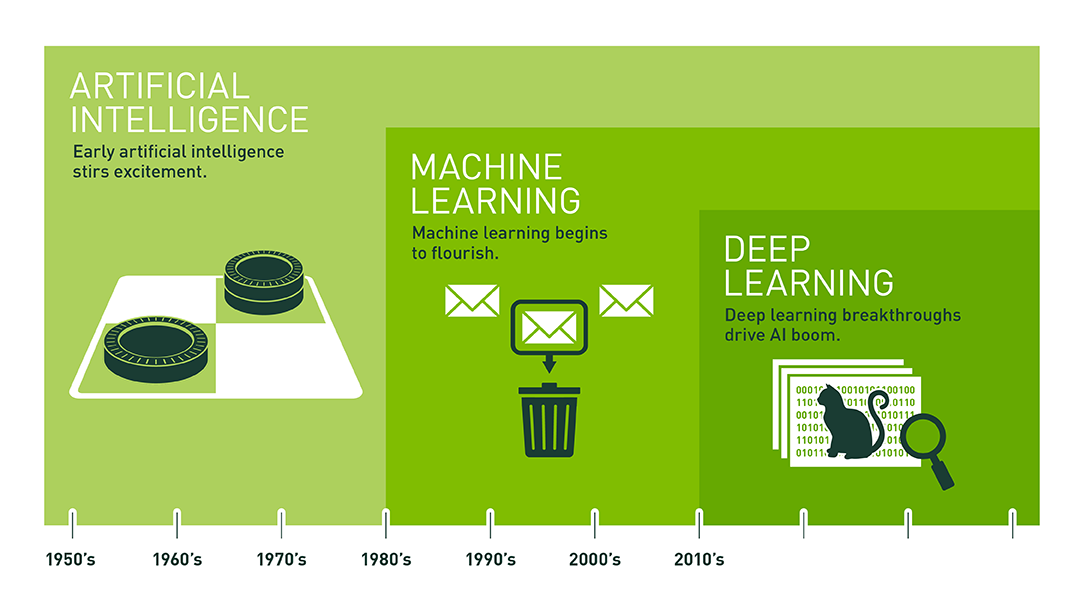
\includegraphics[width=\linewidth]{contents/chapter_3/resources/History.png}
    \caption{Représentation temporelle des différents courant d’intelligence artificielle. L’intelligence artificielle est un courant généraliste, qui comprend les approches par apprentissage ou « machine learning ». Depuis 2010, les approches par apprentissage incluent un nouveau courant : l’apprentissage profond ou « deep learning ». Source : NVidia}
    \label{fig:chapter_3:history}
\end{figure}

\section{Approches analytiques}
Ce terme caractérise, dans le cadre de ce travail, les approches d’intelligence artificielle n’appartenant pas au cadre de l’apprentissage automatique. Il s’agit d’approches dont la succession de règles, ou des traitements pas à pas, est définie par un humain. Cette démarche fait suite aux travaux de Turing, décrivant que tout problème peut se résoudre par une suite d’étapes successives \cite{Turing1937}. L’ordinateur ne cherchera pas à comprendre la relation entre les données d’entrée et attendues en sortie, mais appliquera les divers traitements qui lui ont été demandés.
Ces solutions proposent ainsi des règles statiques et nécessitent une revisite de toute ou partie du processus lorsque les données d’entrées sont vouées à varier. De plus, ces approches peuvent être dépassées en cas d’une grande diversité des données d’entrée.\par
 
\begin{figure}[H]
    \centering
    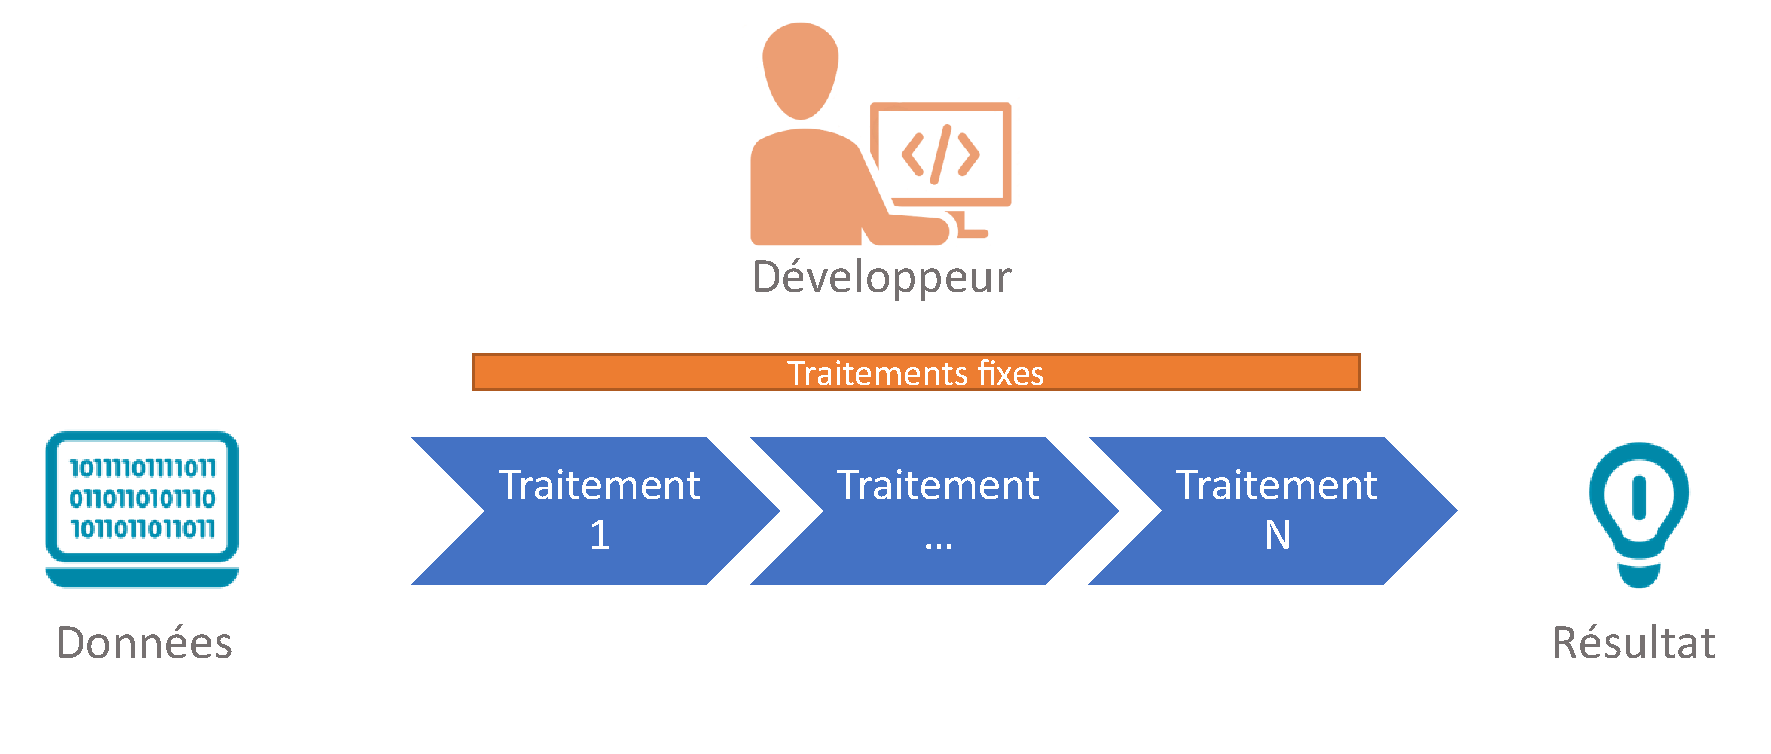
\includegraphics[width=\linewidth]{contents/chapter_3/resources/StandardProcess.pdf}
    \caption{Schématisation d’une approche par algorithme.}
    \label{fig:chapter_3:standard}
\end{figure}
La littérature traitant de « la détection de lésions de la peau » est assez peu développée pour ces approches « algorithmiques » \cite{Moss1989}. Les approches par apprentissage, dont nous allons aborder les grandes lignes dans la section suivante, ont grandement contribué au développement de cette thématique dans la littérature scientifique.\par

\section{Approches par apprentissage}
Ce courant a été « évoqué » en 1948 par Turing A : son idée était de proposer des « machine à apprendre susceptibles de construire elles-mêmes leurs propres codes » \cite{Turing1950}. En 1959, Arthur Samuel  formule une première définition du « Machine Learning » comme étant « domaine d’étude dans lequel nous donnons à l’ordinateur la possibilité d’apprendre sans avoir été explicitement programmé ». Les approches par apprentissage automatique peuvent être résumées aux techniques permettant à un système informatique d’adapter son analyse et son comportement en fonction de ses données d’entrée  . Une définition plus formelle et récente de ce domaine par Tom M. Mitchell  est « qu’un programme informatique apprend d’une expérience E, en adéquation avec des tâches T et une mesure de performance P, si sa performance sur les tâches T, mesurée par P, s’améliore avec l’expérience E ».
Nous pouvons distinguer deux grands courants d’apprentissage, synthétisé dans la Figure 28, dont : 
\begin{itemize}
    \item Le premier courant est exploratoire, également surnommé « approche non supervisée » dans laquelle l’ordinateur tente de trouver des correspondances au sein des données.
    \item Le second courant est prédictif, également appelé « approche supervisée » dans laquelle l’ordinateur tente de faire correspondre des données d’entrée avec des données de sortie attendues. Les prédictions peuvent aboutir à :
    \begin{itemize}
	    \item Des valeurs discrètes : nous parlons d’un problème de classification.
	    \item Des valeurs continues : nous parlons d’un problème de régression.
	\end{itemize}
\end{itemize}

La combinaison de ces deux approches aboutit à une troisième variante dite semi supervisée, permettant d’accroître la précision d’un modèle supervisé par l’ajout de données non labelisées \cite{Murphy2012}.
 
 \begin{figure}[H]
    \centering
    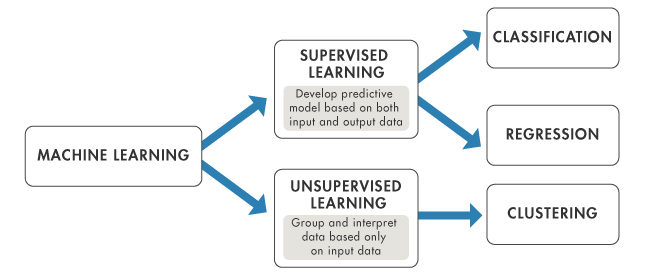
\includegraphics[width=\linewidth]{contents/chapter_3/resources/MachineLearning.png}
    \caption{Machine Learning et sous ensemble. Source : MathWorks}
    \label{fig:chapter_3:machine_learning}
\end{figure}


\section*{Apprentissage supervisé}
L’apprentissage supervisé ou « prédictif » consiste de manière simple à trouver une corrélation entre des données d’entrée x et des sorties attendue y et cela, dans le but de produire sur de nouvelles données d’entrée x' de nouvelles sorties y'.\par
Cette approche implique l’utilisation d’une base d’apprentissage, définie comme « un ensemble de couples entrée-sortie » noté $\{(x_1,y_1 ),…,(x_n,y_n )\}$ avec $n \in N$. Ainsi, l’humain tente de donner une signification aux données utilisées, pour lesquelles la machine sera en mesure de trouver une corrélation.\par
L’algorithme tente de répondre au problème $y=f(x)$ où $f()$ est notre fonction inconnue correspondant au phénomène observé, par une fonction d’approche $g()$ appelée fonction de prédiction, tel que $y=g(x)$.
Cet apprentissage, schématisé en Figure 29, se découpe en deux processus distincts : d’une part, l’entraînement consistant à approcher la fonction $f()$ et d’autre part, la prédiction consistant à évaluer de nouvelles données.\par
  
\begin{figure}[H]
    \centering
    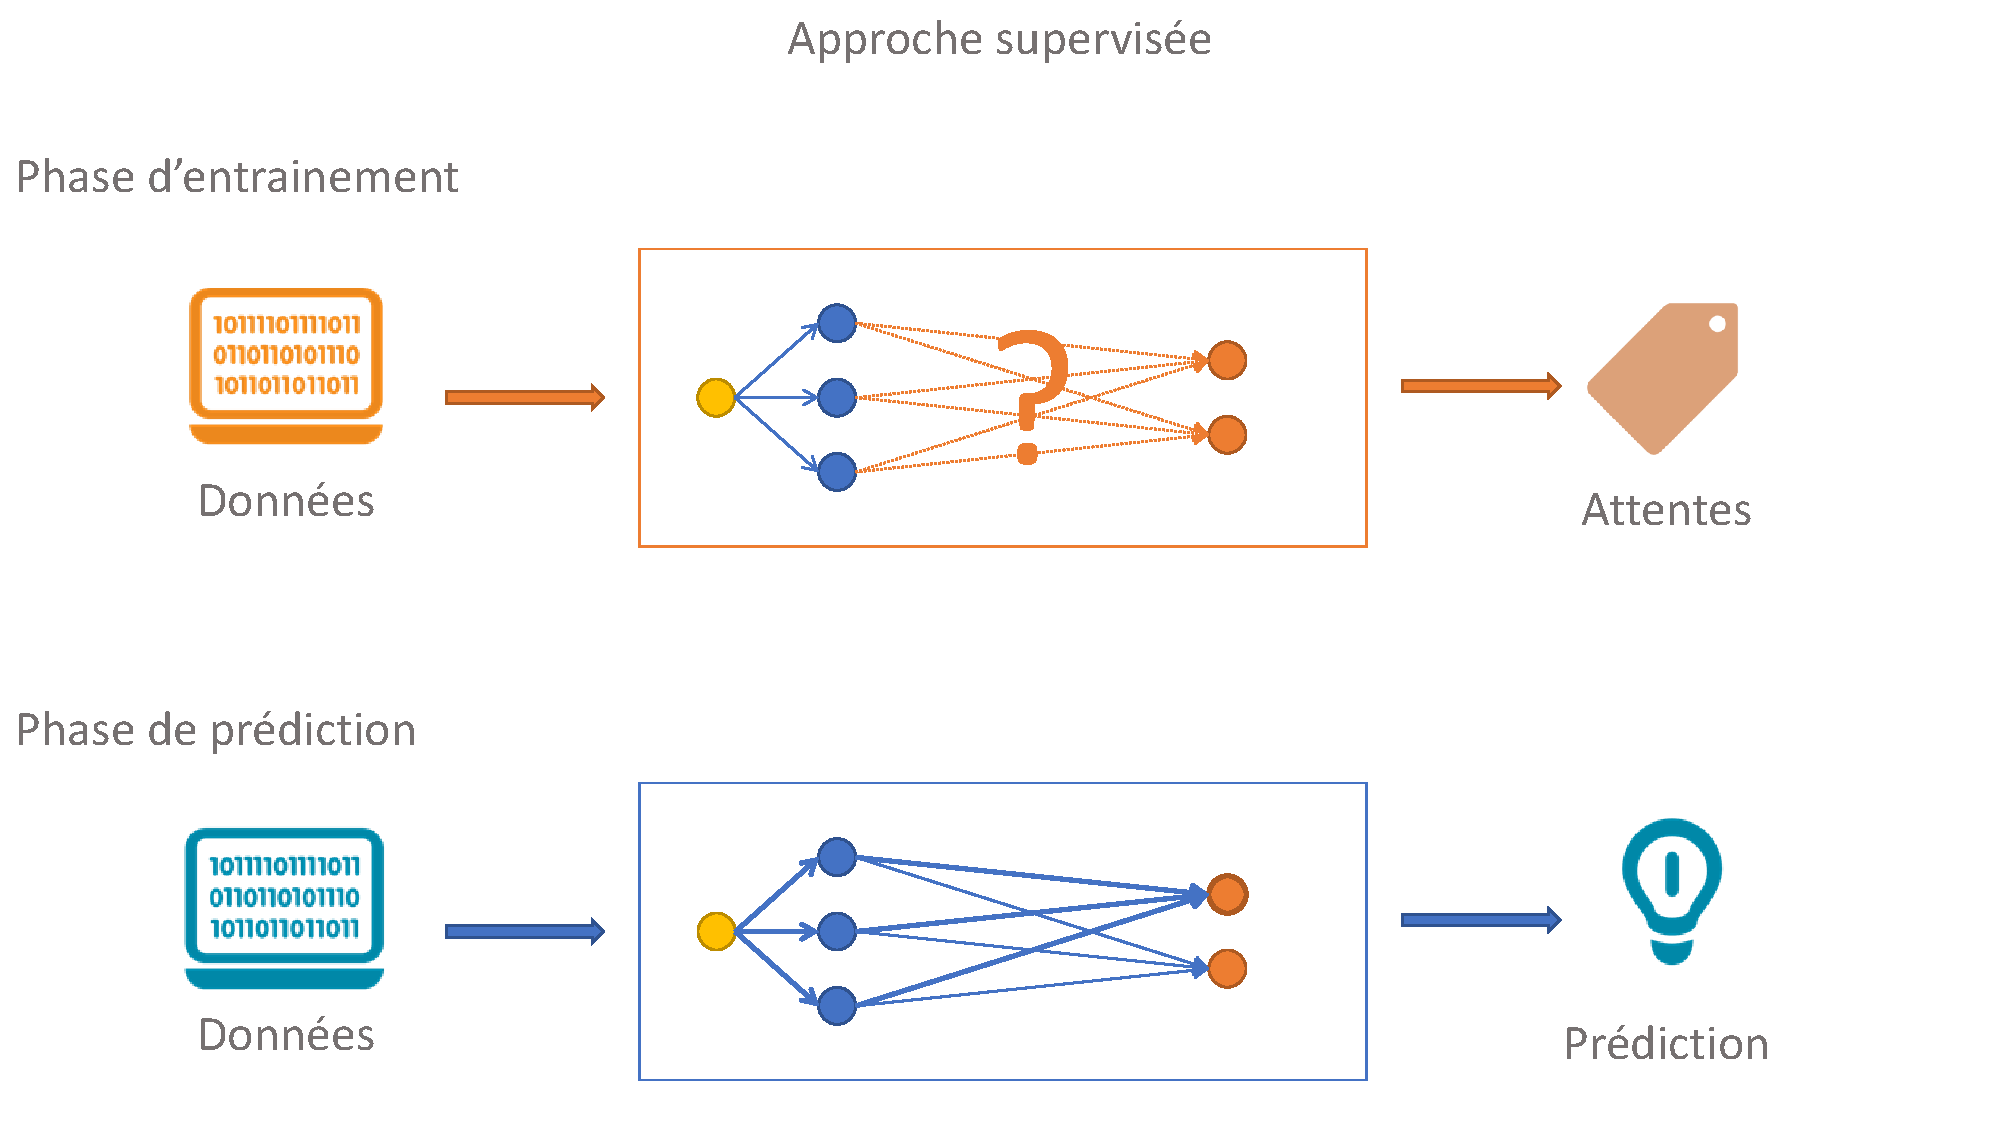
\includegraphics[width=\linewidth]{contents/chapter_3/resources/SupervisedClassification.pdf}
    \caption{Schématisation de l’approche dite supervisée}
    \label{fig:chapter_3:supervised_classification}
\end{figure}

Ces approches se regroupent au travers de deux types majeurs de résolution :
\begin{itemize}
    \item La prédiction de valeurs discrètes soit l’ensemble des entiers relatifs noté $\pmb{\mathbb{Z}}$, désignée sous le terme classification. Cette catégorie se subdivise en deux nouveaux types de classifications, qualifié de binaire ou de multi-classes lorsque la situation nécessite de prédire plus de deux valeurs.
    \item La prédiction de valeurs continues soit l’ensemble des nombres réels noté $\pmb{\mathbb{R}}$, désignée sous le terme de régression.
\end{itemize}\par
	
	

Apprentissage profond
L’apprentissage profond correspond à un sous ensemble des méthodes d’apprentissage automatique qui tentent, par l’apports des neurosciences, de modéliser les schémas de fonctionnement du cerveau humain. Les derniers constats réalisés dans ce domaine, semblent démontrer que le cerveau possède divers niveaux de traitement de l’information . 
En effet, dans le cadre des méthodes « standard » d’apprentissage évoquées dans la partie précédente, la dimension de « couches » de traitement n’est pas intégrée. Les approches par apprentissage simple proposent une architecture en trois couches, dont l’une des couches est allouée à la corrélation entre nos données d’entrée et de sortie. Par opposition, les approches par apprentissage profond proposant des structures en n couches, avec $n \in \pmb{\mathbb{N}}$ et $n>1$. 
Ce choix d’architecture permet l’autodétermination de structures de caractéristiques complexes, définies par une combinaison non linéaire de caractéristiques plus simples. La  Figure 30 met en évidence un cas plus simple de résolution par apprentissage pour appréhender cette notion. 
 
\begin{figure}[H]
    \centering
    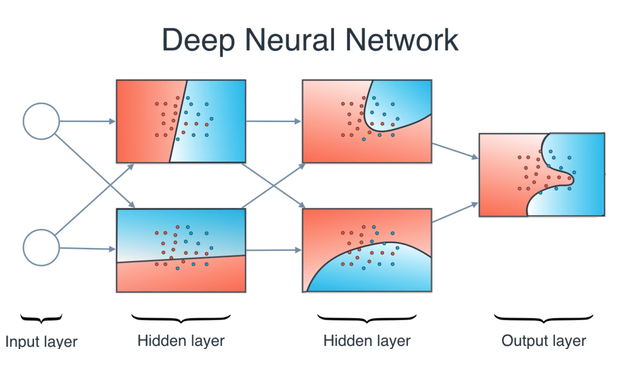
\includegraphics[width=\linewidth]{contents/chapter_3/resources/DeepUnderstanding.png}
    \caption{Exemple simplifié d'une structure d’apprentissage profond. Ce modèle se compose de deux couches intermédiaires cachées : la première couche extrait des caractéristiques linéaires simples, tandis que la seconde couche par combinaison à la première couche conduit à une extraction de caractéristiques plus complexes. Source : Quora}
    \label{fig:chapter_3:deep_understanding}
\end{figure}

Ces solutions ont le désavantage de nécessiter des quantités de données non négligeables ainsi qu’une puissance de calcul, ou a contrario du temps, supérieur aux techniques d’apprentissage « simples ».
Plusieurs travaux ont été menés dans le domaine de la dermatologie pour permettre de déterminer la pertinence de ces méthodes. Nous retiendrons des thématiques autour de la reconnaissance du mélanome [24][25] largement abordé, ainsi que des travaux autour de la classification des lésions de natures diverses [26]. Ce dernier utilise un procédé de transfert de connaissance entre un réseau préalablement entrainé moins spécifique, et un nouveau réseau spécifique au problème de classification des lésions, dans le but de réduire le temps et les ressources nécessaires à l’entrainement du nouveau réseau.
Apprentissage par transfert
L’apprentissage par transfert est une discipline connexe à l’apprentissage profond défini comme « faisant référence à la situation où ce qui a été appris dans un contexte […] est exploité pour améliorer la généralisation dans une autre contexte » [27]. Cette discipline s’inscrit dans le champ de « l’adaptation de domaine », définie comme le transfert des connaissances d’un domaine $D_S$, défini par l’hypothèse $h: X_S \rightarrow Y_S$, vers un domaine cible $D_T$ afin de satisfaire $h: X_T \rightarrow Y_T$.
Ces solutions permettent de réduire les difficultés liées à la grande quantité de ressources de calcul, de temps, mais également de données mobilisées nécessaires à un entrainement depuis sa base. Le modèle d’apprentissage attendu est alors initialement plus performant, croît plus efficacement et plus performant qu’un apprentissage spécifique (Figure 31).

\begin{figure}[H]
    \centering
    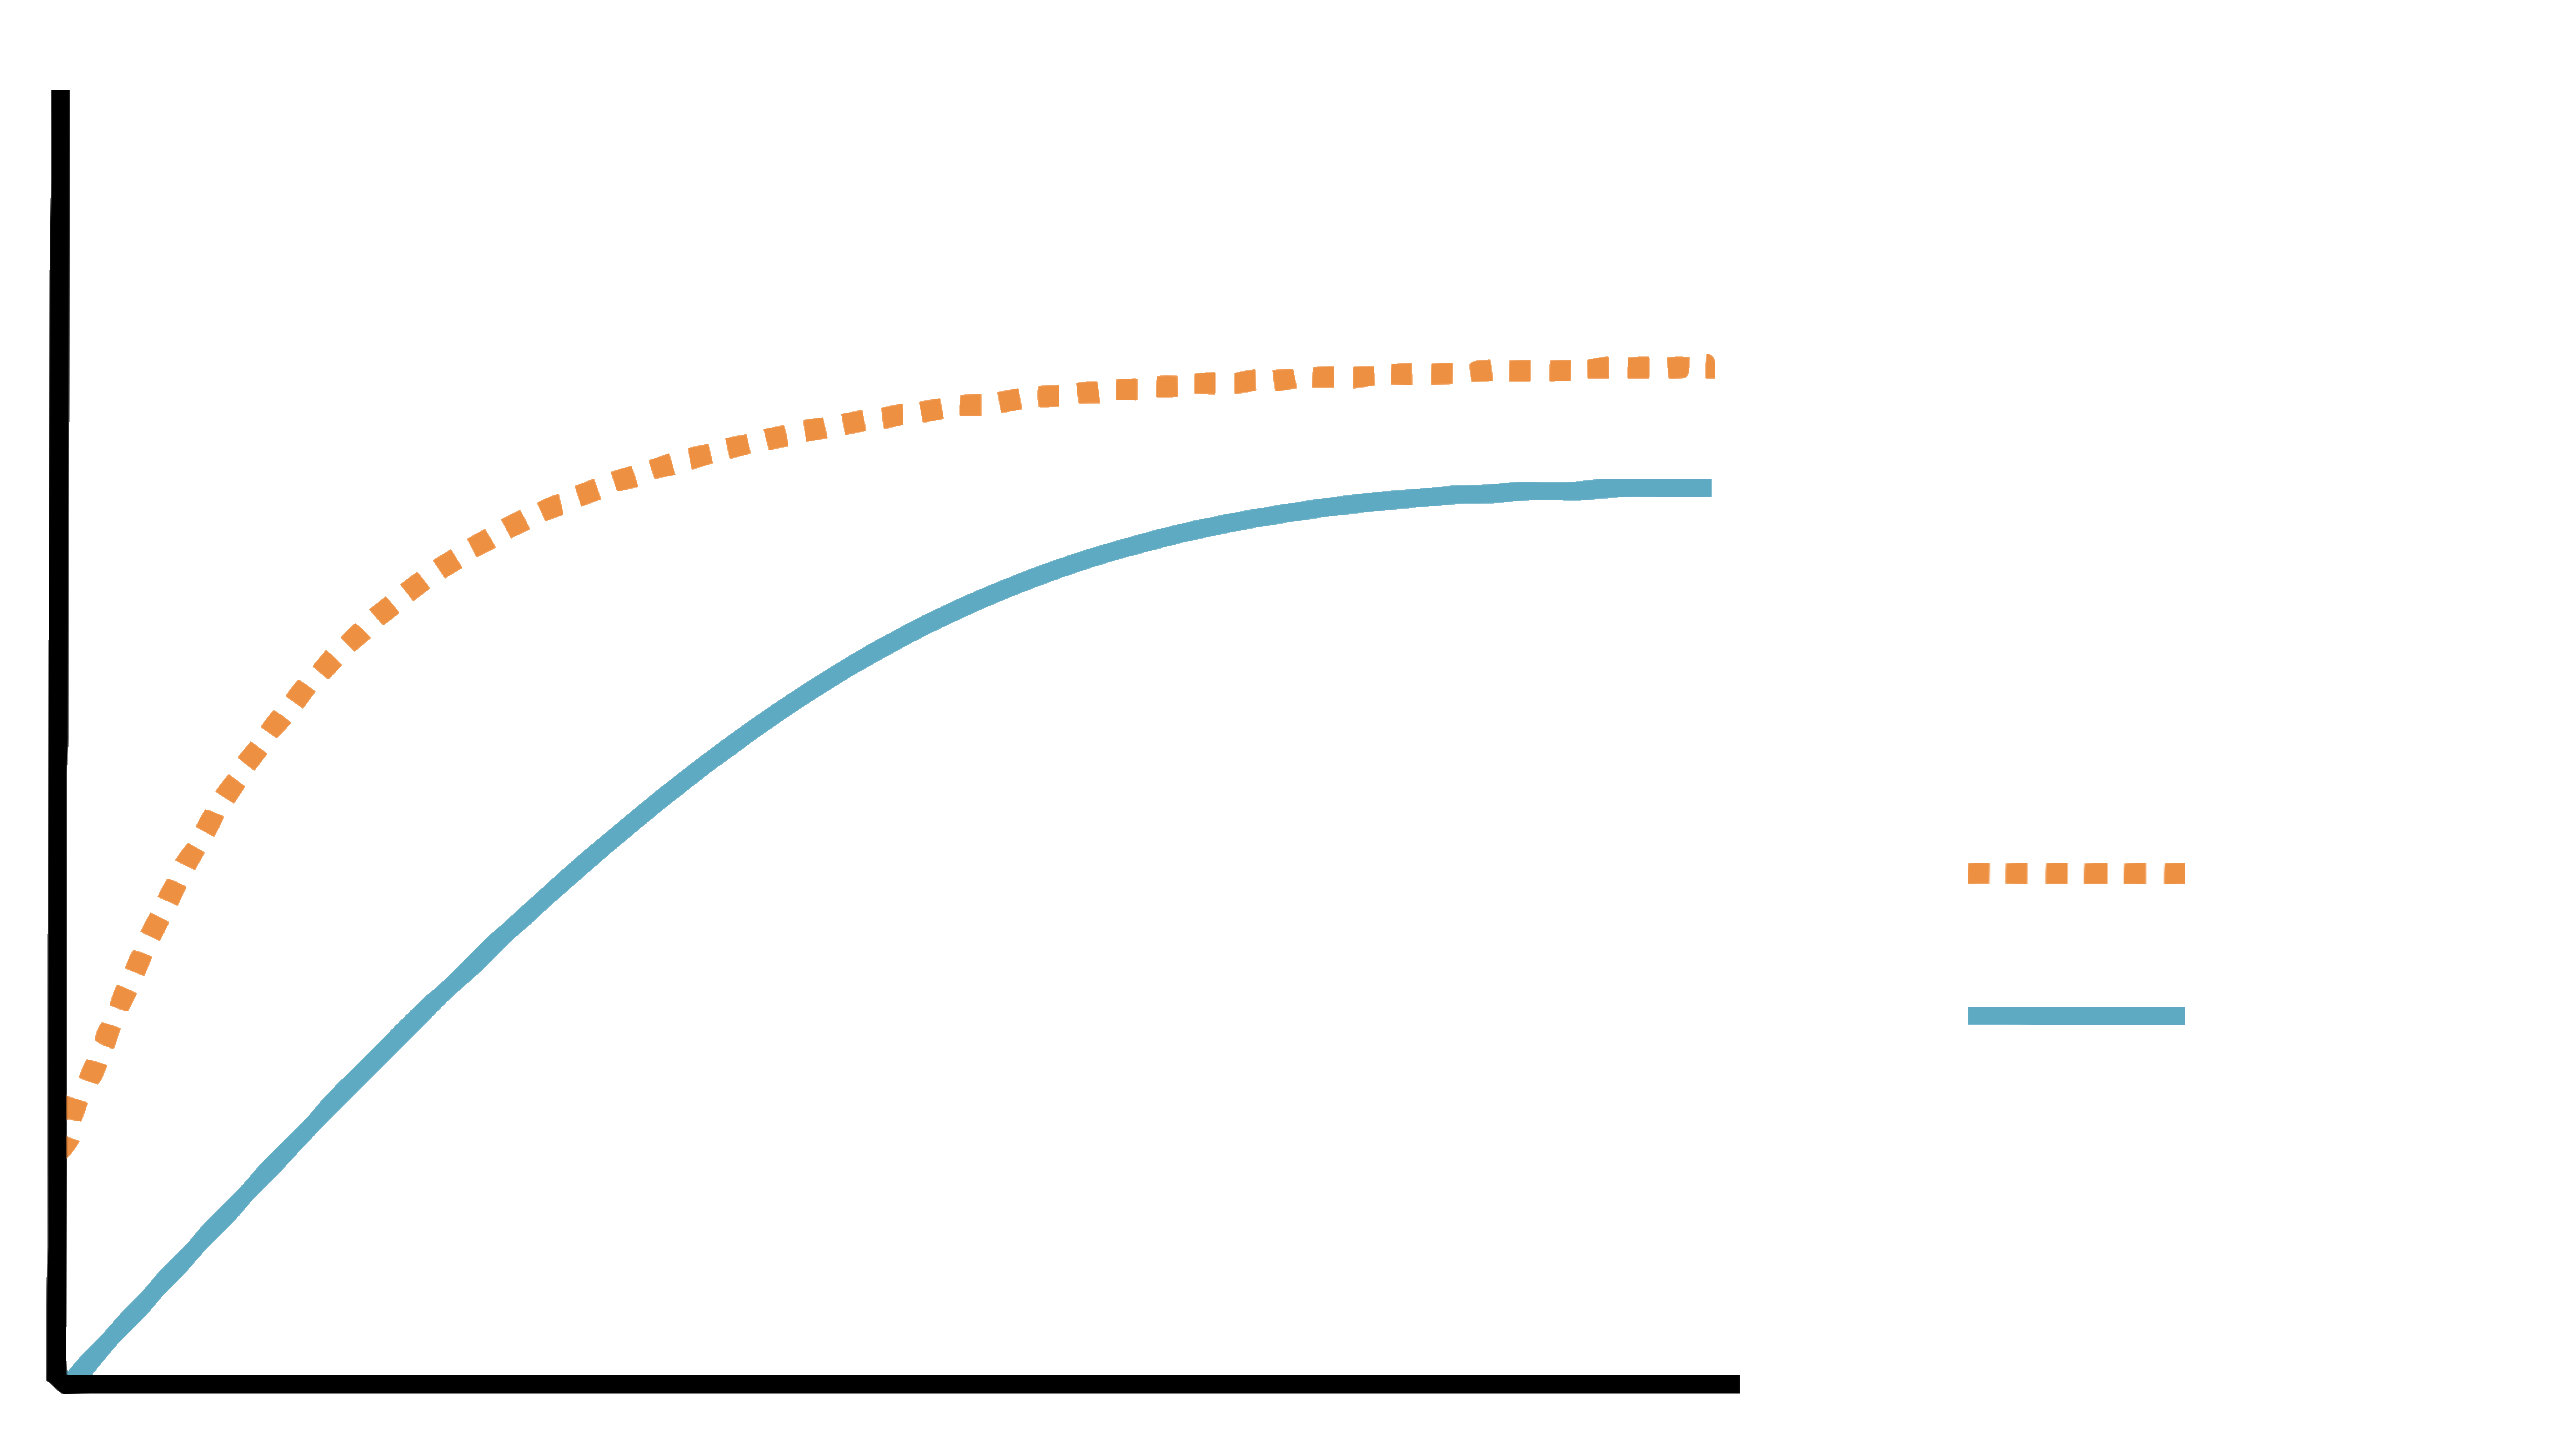
\includegraphics[width=\linewidth]{contents/chapter_3/resources/DeepLearningCurves.png}
    \caption{ Attentes liées à un apprentissage par transfert en opposition à un apprentissage classique. Source : machinelearningmastery.com}
    \label{fig:deep_understanding}
\end{figure}

Néanmoins, cette solution n’est envisageable que lorsque l’apprentissage, réalisé lors de la première tâche, généralise suffisamment le phénomène observé. Ainsi, il est d’usage courant de ne spécifier lors du transfert que la couche finale de classification du réseau, les premières couches n’étant employé comme extracteur général de caractéristiques. Toutefois, la littérature s’accorde sur une possible spécialisation des couches de classification et hautes moins génériques (Figure 32).
   

\section{Apprentissage non supervisée}
L’apprentissage non supervisé ou « descriptif » est une seconde approche d’apprentissage dans laquelle l’ordinateur tente de « découvrir » en autonomie, des corrélations au sein de jeux de données. Ces approches émergent de problématiques diverses, telles que :
	Réduire le coût, ou temps humain nécessaire, d’obtention de données labellisées, c’est-à-dire pour lesquelles le couple de données d’entrée et de sortie attendue est connu.
	Découvrir les diverses relations pouvant exister au sein d’un amas de données. En effet, un label n’est qu’un échantillonnage de l’information primaire, et ne permet pas d’obtenir les relations pouvant régir des modèles complexes.
	Explorer de nouvelles relations de type « cause – effet », en réaction à la masse de données produites par les objets connectés. 

Plusieurs applications existent, telles que :
	Le regroupement par classes, des algorithmes comme les k-moyennes tentent de minimiser la différence d’énergie entre les points d’un même groupe.
	La réduction de dimensions sur des données à grande complexité, par projection de ces dernières sur des espaces à dimension réduite. On souhaite par ce procédé garder l’information essentielle au processus décisionnel.
	La découverte de relations au sein de l’information, et des relations les plus robustes entre variables et dépendances.
 
\begin{figure}[H]
    \centering
    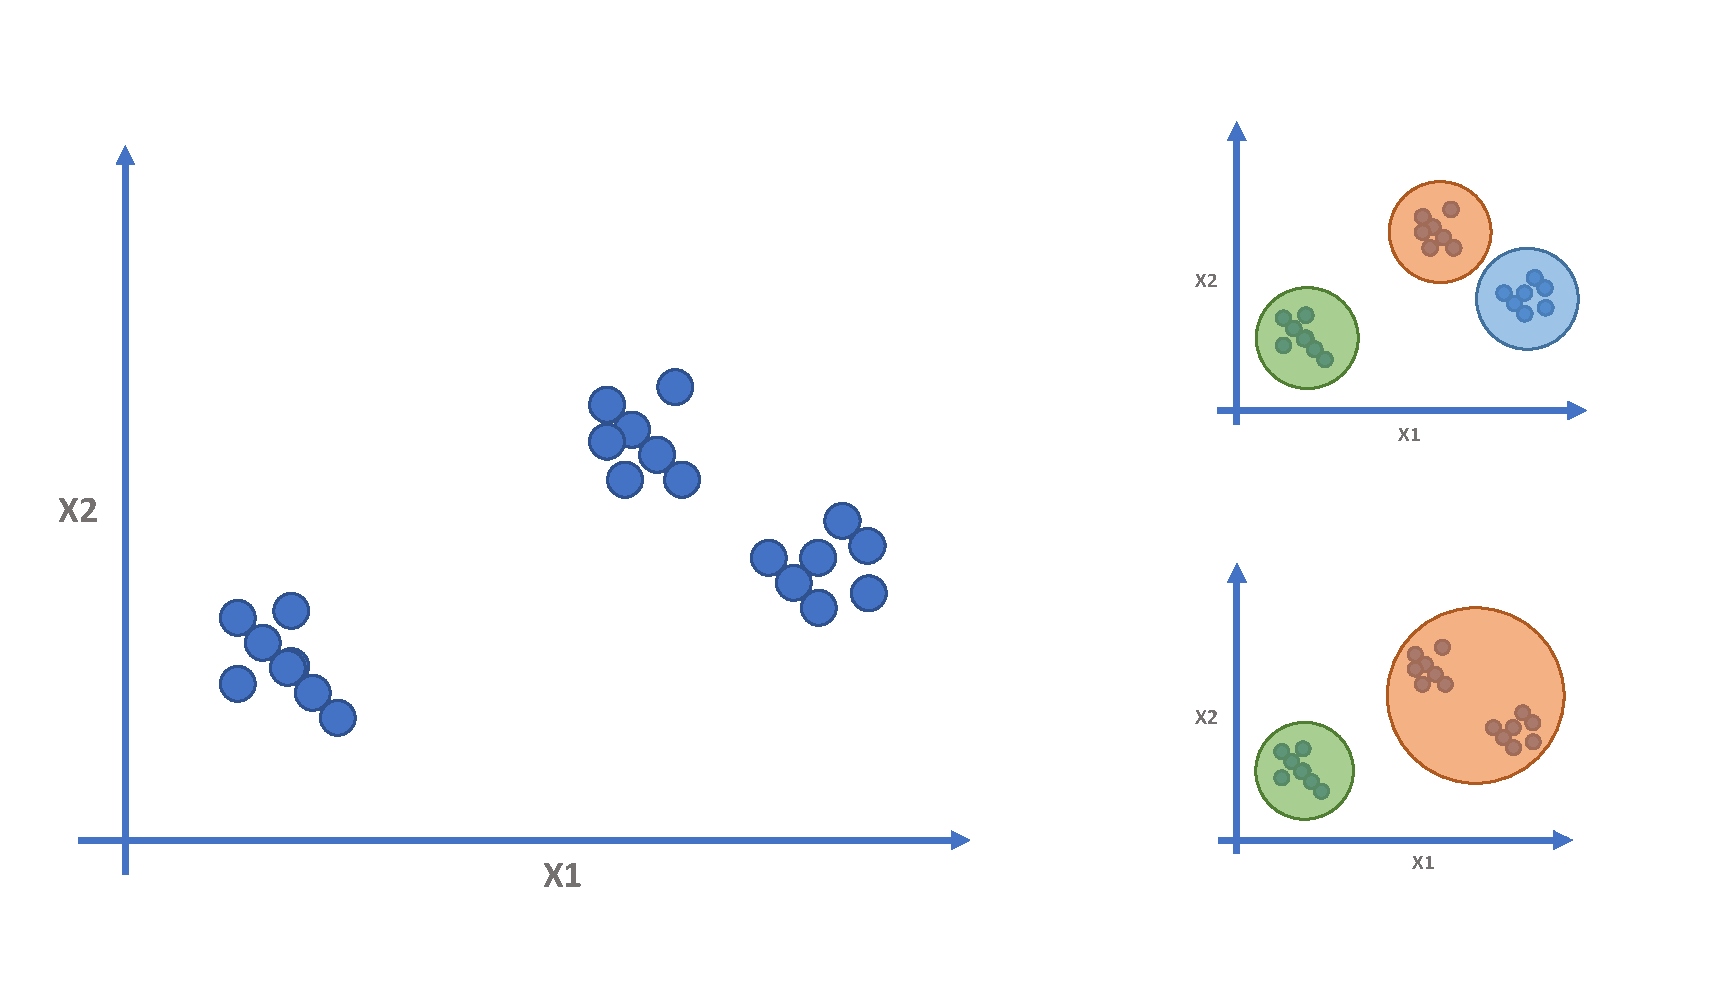
\includegraphics[width=\linewidth]{contents/chapter_3/resources/Unsupervised.pdf}
    \caption{Les données fournies ne sont pas associées à un label attendu. Nous demandons à la machine de découvrir des groupes de données (exemple avec 2 groupes et 3 groupes).}
    \label{fig:chapter_3:unsupervised}
\end{figure}

Cette partie a pour but d’aborder les techniques en dehors des deux précédentes catégories. Il peut s’agir de techniques hybrides ou n’appartenant pas de manière significative aux deux précédentes classes. 

\section{Autre}
\subsection{Apprentissage semi supervisé}
Ces techniques tentent de combiner les deux principes précédents. Il est généralement difficile d’obtenir des données en suffisance correctement labellisées. D’une part, cela requiert le travail d’un opérateur sur ces données afin d’y associer les annotations adéquates. D’autre part, un grand nombre de données implique un possible biais humain dû à des erreurs sur ces annotations (manque d’attention, mauvaise interprétation de la donnée, …).
Les données labellisées permettent de définir des groupes spécifiques au sein de ces données, tandis que les données non labellisées, en plus grande quantité, permettent d’affiner les limites des groupes préalablement détectés (Figure 34). Différentes techniques existent, basées sur des critères tels que la densité de l’information labellisé et non labellisé [28], pouvant s’apparenter à une forme de clustering.
 
\begin{figure}[H]
    \centering
    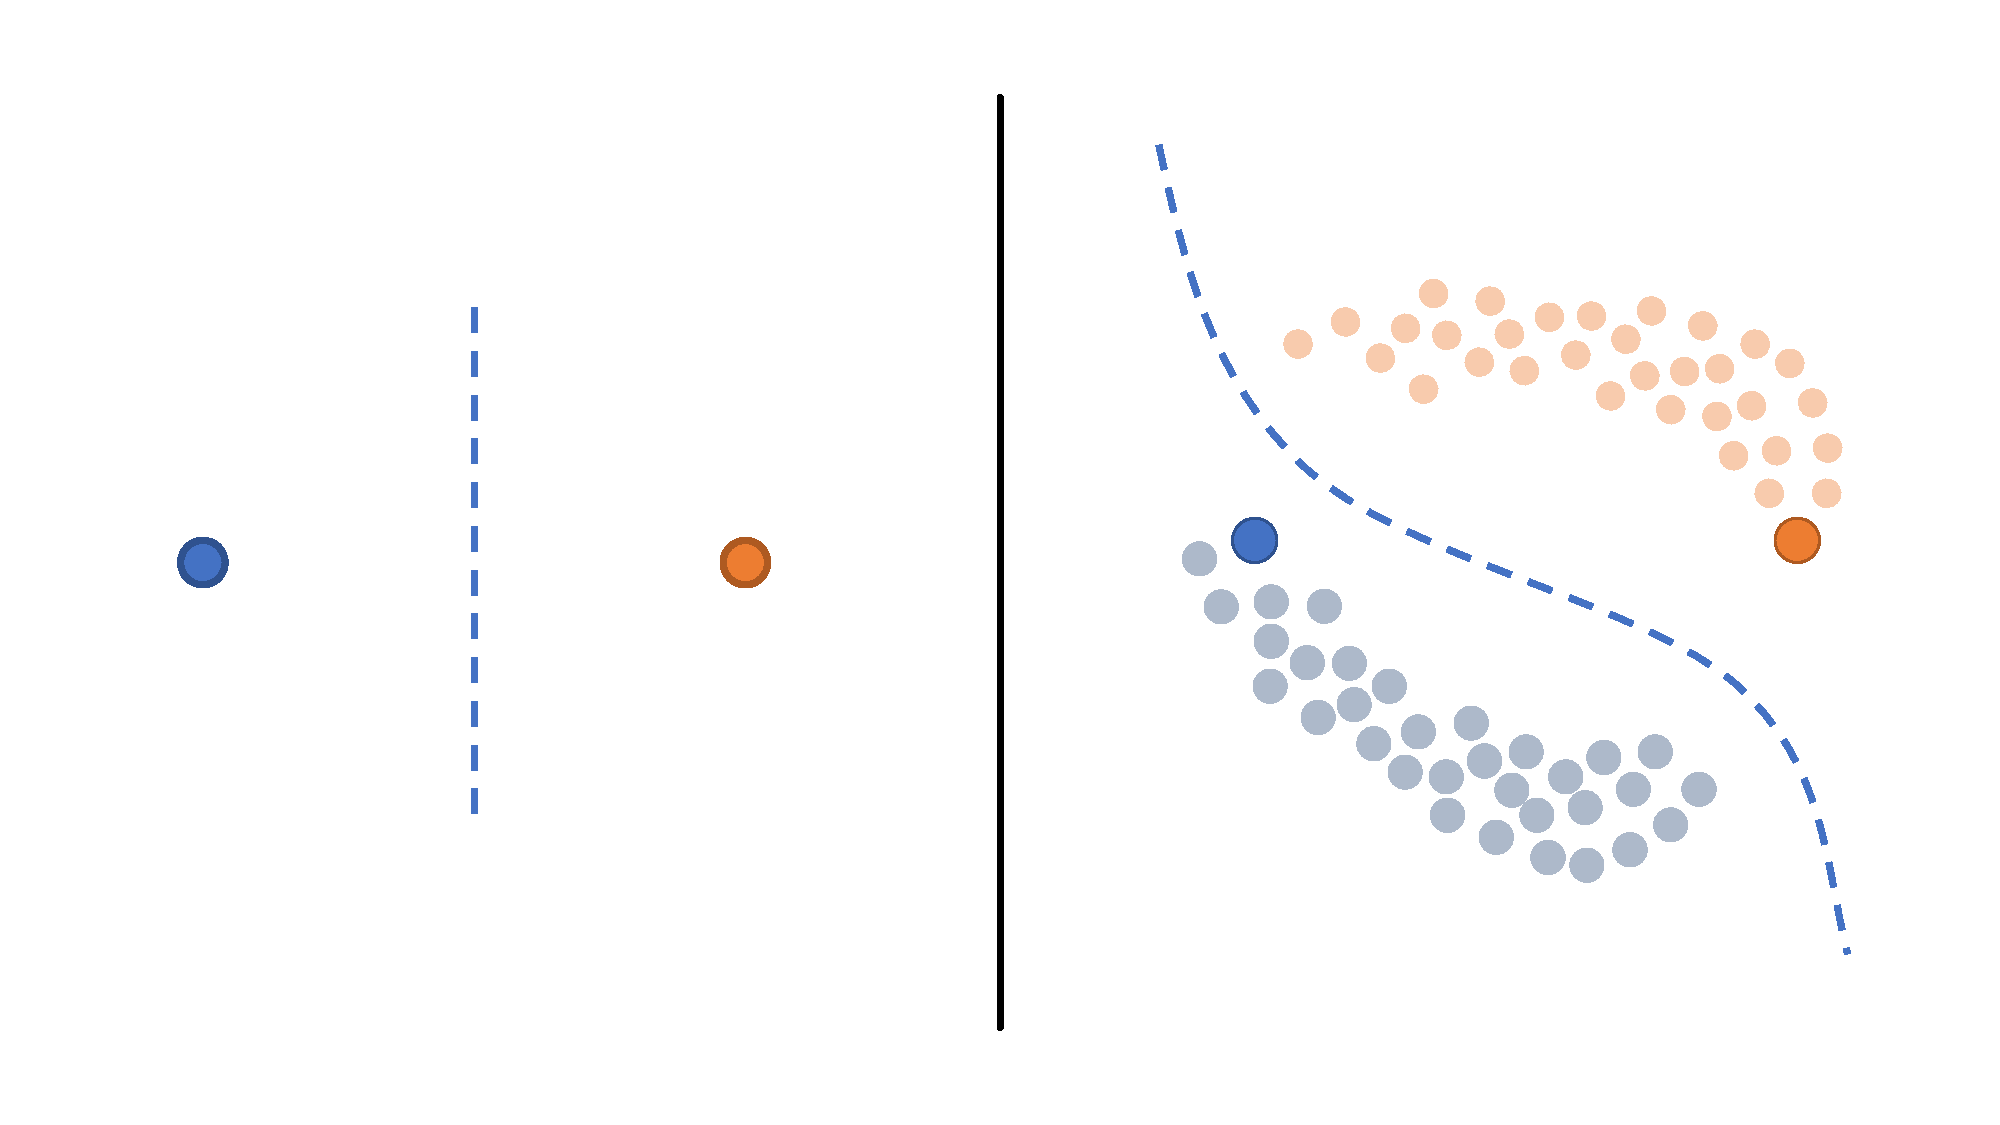
\includegraphics[width=\linewidth]{contents/chapter_3/resources/Semisupervised.pdf}
    \caption{A gauche, une classification obtenue à partir de deux données labellisées, à droite ces mêmes données avec l’ajout de données non labellisés. Ces nouvelles données sont alors attribuées à l’une ou l’autre des classes.}
    \label{fig:semisupervised}
\end{figure}

\subsection{Détection de valeurs aberrantes / anomalies}
Cette technique est particulièrement propice aux données représentant majoritairement les cas définis comme « normaux », et pour lesquels nous souhaitons détecter les cas « aberrants ». En 1980, Douglas Hawkins apporte la définition d’une valeur aberrante comme « Une observation qui s’écarte tellement des autres observations, qu’elle éveille le soupçon d’avoir été généré par un mécanisme différent ». Diverses méthodes existent, dont l’une des plus utilisées se base sur une distribution gaussienne, excluant les valeurs qualifiées d’extrême déterminée par un seuil $\varepsilon$ (Figure 35). Gaussian mixture model.
  
\begin{figure}[H]
    \centering
    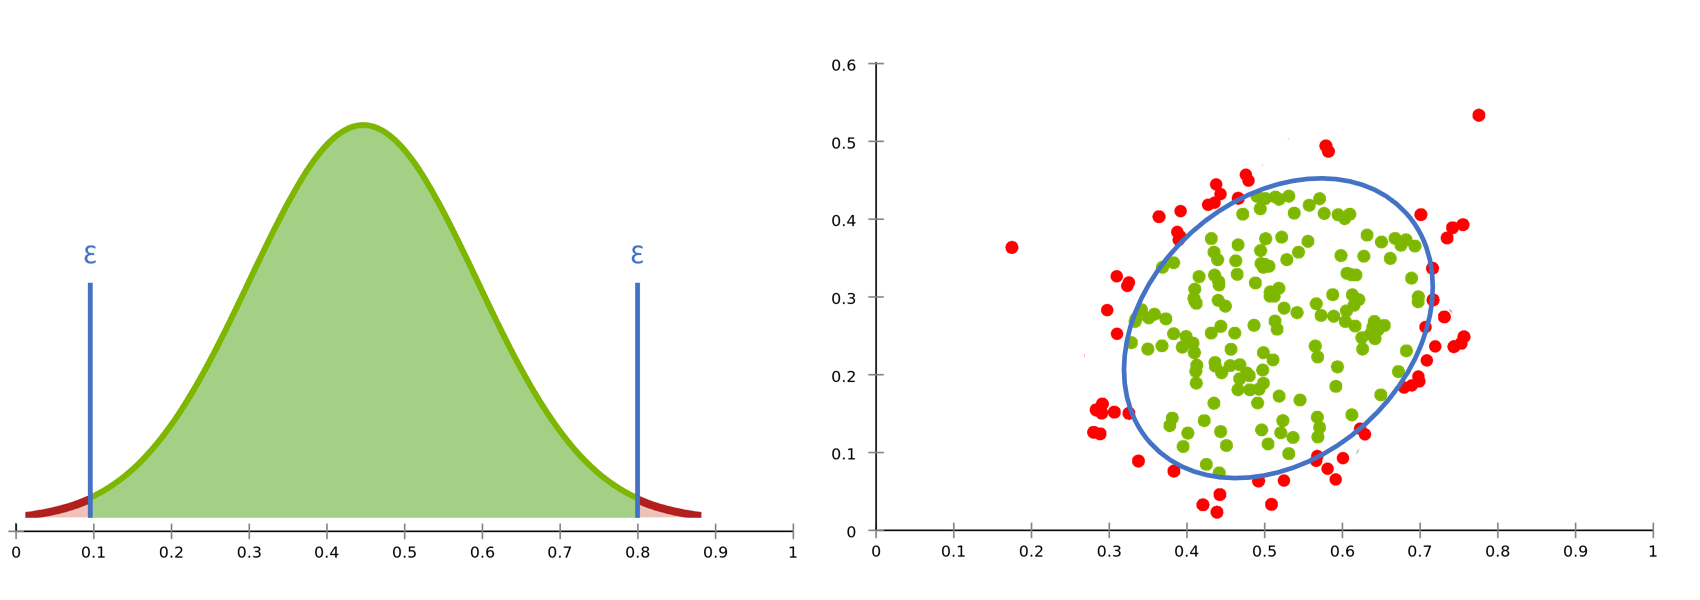
\includegraphics[width=\linewidth]{contents/chapter_3/resources/AnomalyDetection.png}
    \caption{Exemple sur des données arbitraires. Un seuil $\varepsilon$ (en bleu) est déterminé à partir des moyennes et écart type des données.}
    \label{fig:anomaly}
\end{figure}

\subsection{Problématiques}
Cette partie se concentre sur des problématiques pouvant engendrer un biais lors de la génération de modèle par ces approches d’apprentissage. Nous tenterons de voir ces problèmes indépendamment et comment y remédier.

\subsubsection{Choix de métriques}
Les métriques sont une part de nos problématiques lors de la mise en place de modèle d’apprentissage. Ces métriques permettent de répondre à deux questions, d’une part « Quel modèle choisir ? » en mettant à notre disposition un critère de comparaison et d’autre part, « Quelle est l’efficacité obtenue ? » en nous permettant d’évaluer la pertinence du modèle retenu.
L’un des premiers outils à disposition est la matrice de confusion (Figure 36), permettant de mettre en avant la performance des prédictions. La matrice diagonale fait figurer les prédictions correctement réalisées par notre modèle, tandis que les éléments restants nous renseignent sur les mauvaises prédictions. Cette matrice fait ainsi ressortir 4 valeurs :
	Les vrais positifs, les éléments de la classe positive détectés comme positif.
	Les vrais négatifs, les éléments de la classe négative détectés comme négatif.
	Les faux positifs, les éléments de la classe négative détectés comme positifs.
	Les faux négatifs, les éléments de la classe positive détectés comme négatifs.

\begin{figure}[H]
    \centering
    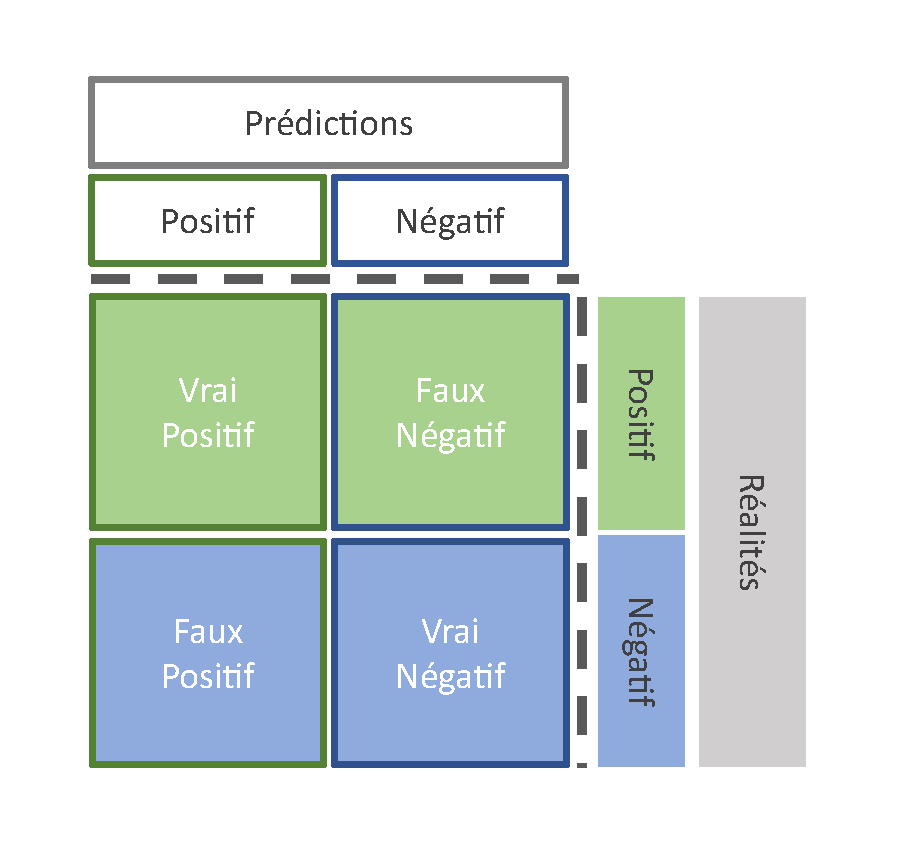
\includegraphics[width=\linewidth]{contents/chapter_3/resources/ConfusionMatrix.pdf}
    \caption{Schéma représentatif d’une matrice de confusion binaire, avec une classe dite positive et une classe dite négative.}
    \label{fig:chapter_3:confusion_matrix}
\end{figure}

Pour répondre à cette problématique, diverses métriques seront à envisager selon la problématique à laquelle nous tenterons de répondre. Ainsi, dans une classification binaire les critères de sensibilité et spécificité seront à considérer, tel que souvent employé dans le domaine. La moyenne fait également partie des critères extrait, mais il est néanmoins important de considérer les cas de non balancement des données pouvant fortement influencer ce paramètre (Équation 1)[29]. 

\begin{equation} 
    \label{eq:chapter_3:Metrics}
    \begin{split}
    &Sensibilité=  TP/(TP+FP) \\	
    &Moyenne=(TP+TN)/(TP+TN+FP+FN) \\
    &Spécificité=  TN/(TN+FN) \\
    &Précision=TP/(TP+FP)
    \end{split}
\end{equation}

Il peut être préférable de privilégier des métriques plus robustes, dans le cadre de données non balancées. Dans ces cas, les sources s’accordent à l’utilisation de métriques tels que le F-Score, associant conjointement sensibilité et précision (principe de la moyenne harmonique, voir Équation 2), ou d’aire sous la courbe (AUC), associant sensibilité ainsi que spécificité et intégrant une indépendance vis-à-vis de seuils de classification (Figure 37).\par

\begin{equation} 
    FScore=(1+\beta²)*(Précision*Sensibilité)/((\beta^2*Précision )+Sensibilité)
    \label{eq:FScore}
\end{equation}


Bien entendu, les scores dépendront du caractère souhaité pour notre classifieur, en minimisant la sensibilité ou spécificité dans le cadre du FScore par exemple. Ce que l’indépendance de l’AUC ne permet pas.\par
 
\begin{figure}[H]
    \centering
    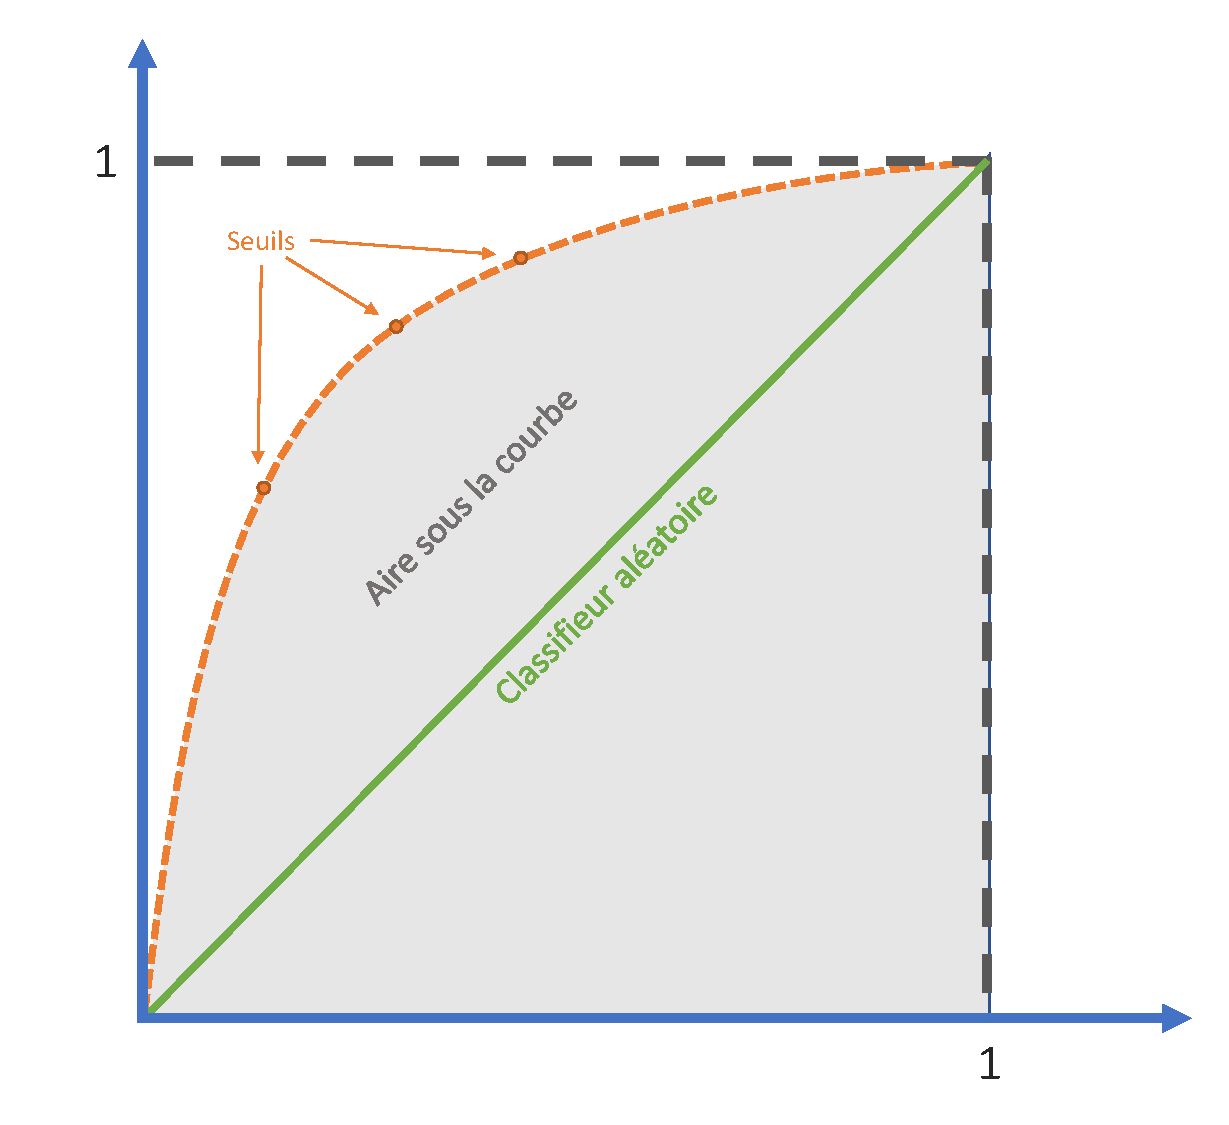
\includegraphics[width=\linewidth]{contents/chapter_3/resources/RocCurve.pdf}
    \caption{Courbe ROC (Receiver Operating Characteristic) et AUC.}
    \label{fig:chapter_3:roc}
\end{figure}

\subsubsection{Equilibrage de données}
Nous regroupons au travers de ce terme l’ensemble des problématiques relatives à notre jeu de données et à la représentation de ses classes. Dans le cas de pathologie de la peau, cela peut se caractériser par un jeu de données composé de 100 éléments dont 20\% d’entre elles se réfèrent à des patients atteints de mélanomes et le reste à des patients sains. Nous constatons dans ce cas un déséquilibre entre les classes de ce jeu de données, qu’il nous faudra prendre en compte. Un tel jeu de données peut être qualifié de « non balancés », la répartition de ses classes n’étant pas égale en proportions.
En effet, certains algorithmes de prédictions peuvent être biaisés, comme par exemple « l’algorithme des plus proches voisins » qui se composera de zones de forte densité privilégiant les données présentes en masse (exemple Figure 37). Un autre biais est également présent lors de l’extraction de métriques pour juger de la pertinence d’un modèle. En effet, dans le cas d’un classifieur qui prédirait constamment « sain », nous obtiendrons un score de 80\% de précision sur notre jeu de données précédent.
  
\begin{figure}[H]
    \centering
    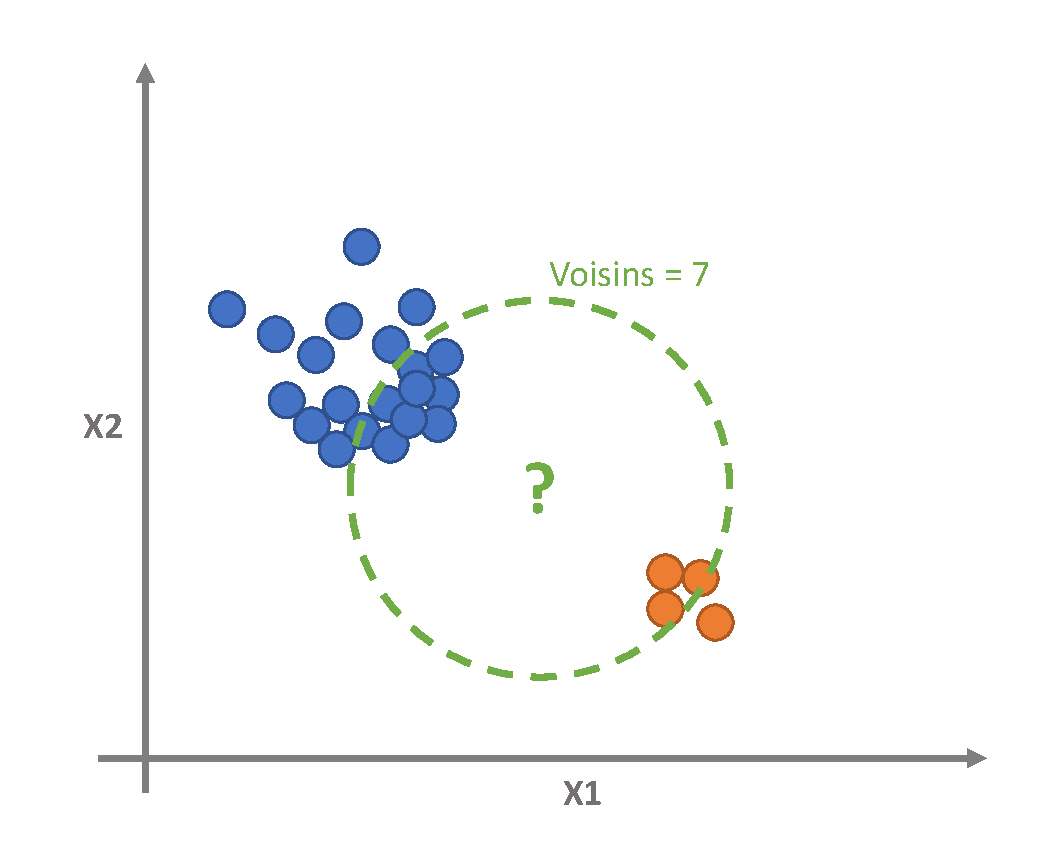
\includegraphics[width=\linewidth]{contents/chapter_3/resources/Unbalanced.pdf}
    \caption{Illustration du problème de données non balancées sur l’algorithme KNN. La densité des données bleu étant supérieure, des prédictions à la frontière de nos deux classes favorisent la classe bleue.}
    \label{fig:chapter_3:Unbalanced}
\end{figure}

Plusieurs méthodes existent dans la littérature, pour permettre de rétablir l’équilibre entre les différentes classes. Nous pouvons citer les deux principaux :
	Le sur-échantillonnage, c’est-à-dire que nous gonflons les classes sous représentatives de manière à égaliser la population de la classe majoritaire (en créant de nouveaux éléments artificiels par exemple).
	Le sous-échantillonnage, c’est-à-dire que nous réduisons la population de l’ensemble des classes à celle de la classe minoritaire.
 
\begin{figure}[H]
    \centering
    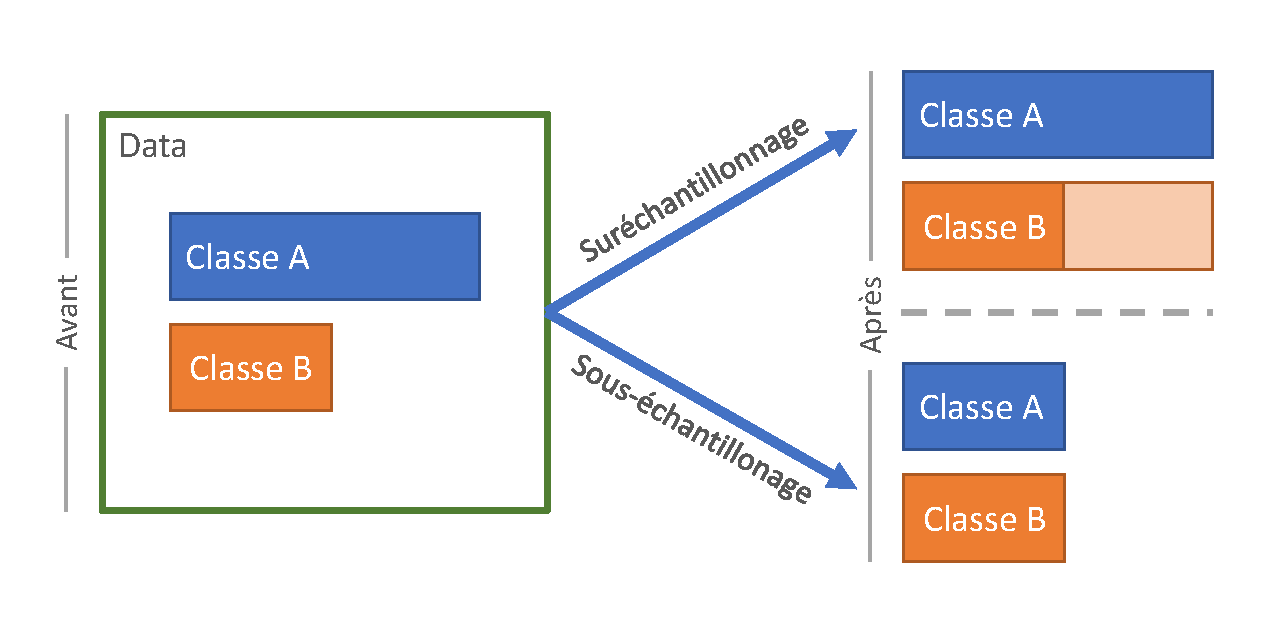
\includegraphics[width=\linewidth]{contents/chapter_3/resources/BalancementStrategies.pdf}
    \caption{Représentation de deux principales catégories de stratégie de balancement des données. Le suréchantillonnage tente d’augmenter la taille du jeu de données faible tandis que le sous échantillonnage tend à réduire la classe majoritaire. }
    \label{fig:chapter_3:Balancement}
\end{figure}

\subsubsection{Vers une généralisation de modèle}
Pour assimiler cette problématique, il est nécessaire de bien comprendre le cheminement de ce type d’approche. En effet, à l’aide de couples de données entrée-sortie (données d’entrainement), nous allons tenter d’apprendre une relation / un modèle capable d’estimer de nouvelles sorties sur de nouvelles données (différentes de celles d’entrainement). 
L’information traitées peut être ainsi plus ou moins aisément séparable, en cause souvent la qualité de(s) l’hypothèse(s) posée(s), du bruit, … L’objectif est de produire un modèle capable :
	De généraliser, et d’être à même de traiter de nouveaux cas 
	D’être spécifique, et de comprendre l’information traitée.
Ce problème, évoqué dans la littérature porte le nom de « Dilemme biais / variance » , dans lequel le biais représente le manque de relation pertinente entre données d’entrées et de sorties et où la variance représente l’influence du modèle au petites fluctuations souvent issues de bruit. Ces termes sont intrinsèquement liés aux problématiques respectives de sous apprentissage et sur apprentissage. La Figure 39 reprend de manière visuelle ces problématiques, et les exprime selon un jeu d’entrainement et de test. A noter que le surapprentissage peux être limité par l’utilisation de termes de régularisation, de schéma de validation de modèle adaptés ou l’utilisation d’ensembles de donnés suffisantes. 
 
\begin{figure}[H]
    \centering
    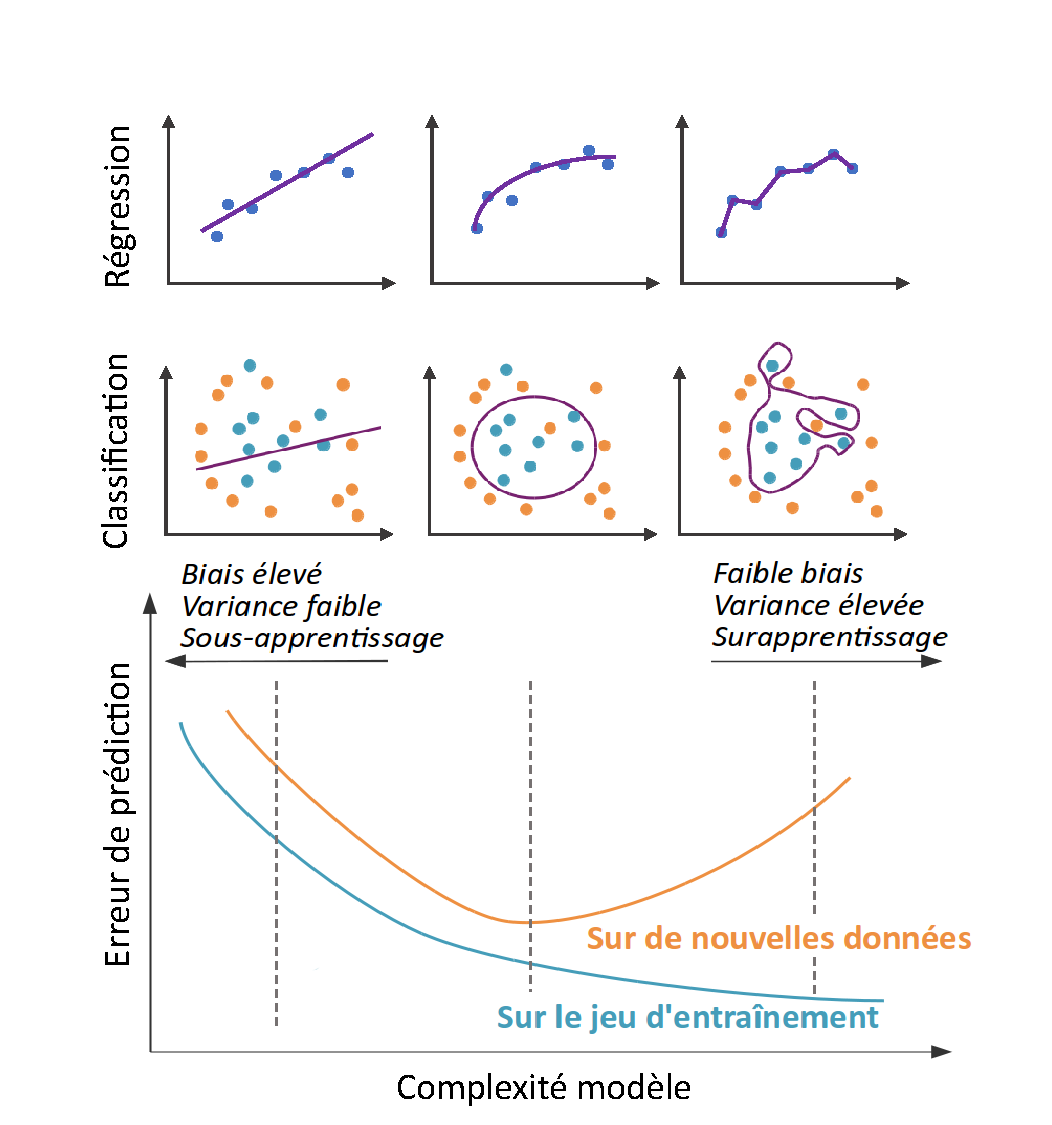
\includegraphics[width=\linewidth]{contents/chapter_3/resources/UnderfitOverfit.pdf}
    \caption{Exemple de dilemme Biais/Variance. L’exemple de gauche représente un cas de sous apprentissage / biais, ce modèle est une sous approximation du phénomène observé. A contrario, l’exemple de droite représente un cas de sur apprentissage / variance, le modèle ne généralise pas suffisamment le phénomène observé. Source : Inspirée OpenClassroom }
    \label{fig:chapter_3:UnderfitOverfit}
\end{figure}

\subsubsection{Évaluation de modèles}
L’élaboration d’un algorithme de prédiction ne se résume pas à sa construction. En effet, il est important d’obtenir un indice permettant de renseigner sur la fiabilité de ce modèle et de ses prédictions futures dans des situations où la vérité terrain ne sera pas connue. L’un des mécanismes les plus simples (holdout method) consiste à diviser l’échantillon de données en deux sous-ensembles, dont les ratios représentatifs de chaque classe seront équivalents pour la classification. L’un des ensembles sert d’entrainement tandis que le second de test (Figure 40). Les données restent ainsi non utilisées jusqu’au moment de la validation, où les prédictions sur le jeu de test sont confrontées à leur réalité terrain. Ces données de test doivent être représentatives des données futures que traitera le modèle afin que cette métrique soit pertinente.

\begin{figure}[H]
    \centering
    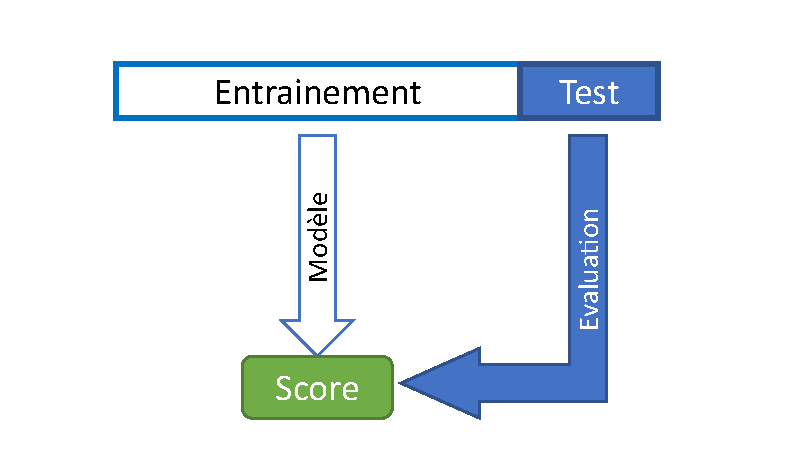
\includegraphics[width=\linewidth]{contents/chapter_3/resources/Holdout.pdf}
    \caption{Principe de la méthode « holdout ».}
    \label{fig:chapter_3:Holdout}
\end{figure}

Afin de d’établir un score plus pertinent, il est de coutume de procéder à une validation croisée de notre modèle. Le jeu de données est subdivisé ainsi en k blocs, servant à tour de rôle de jeu d’évaluation et le reste d’entrainement. Nous obtenons ainsi k scores, que nous utiliserons pour déterminer le score final par moyenne de ceux-ci (Figure 41).
 
 \begin{figure}[H]
    \centering
    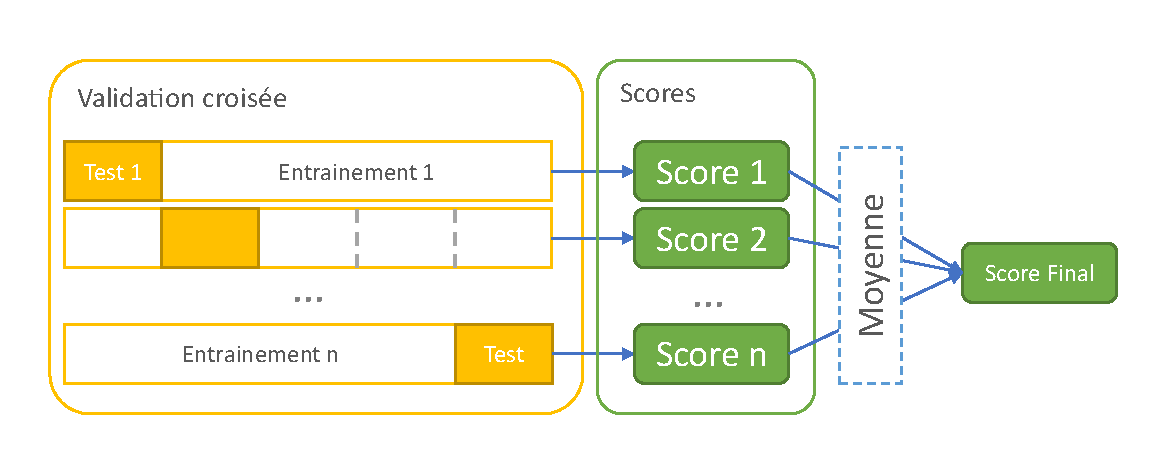
\includegraphics[width=\linewidth]{contents/chapter_3/resources/CrossValidation.pdf}
    \caption{Principe de l’évaluation par validation croisée.}
    \label{fig:chapter_3:CrossValidation}
\end{figure}

\subsubsection{Réglages Hyper paramètres}
Avant d’entrer plus en profondeur dans le sujet, il est nécessaire de revenir au terme « d’hyper paramètres ». Ce terme caractérise les paramètres dont le réglage s’effectue avant le processus d’apprentissage, tandis que les autres paramètres découlerons de l’entrainement.
Le paramétrage de ces paramètres est le plus souvent difficile à appréhender, et dépendra fortement de la situation rencontrée. Il est donc nécessaire de procéder à leur réglage par comparaison entre différentes valeurs. L’une des techniques courantes consiste à définir une « grille » (cube, hypercube, … selon le nombre de paramètres) contenant une variation de ces valeurs selon un axe. Nous tenterons d’extraire la combinaison de paramètres capables de fournir les meilleurs résultats comme dans la Figure 42.

\begin{figure}[H]
    \centering
    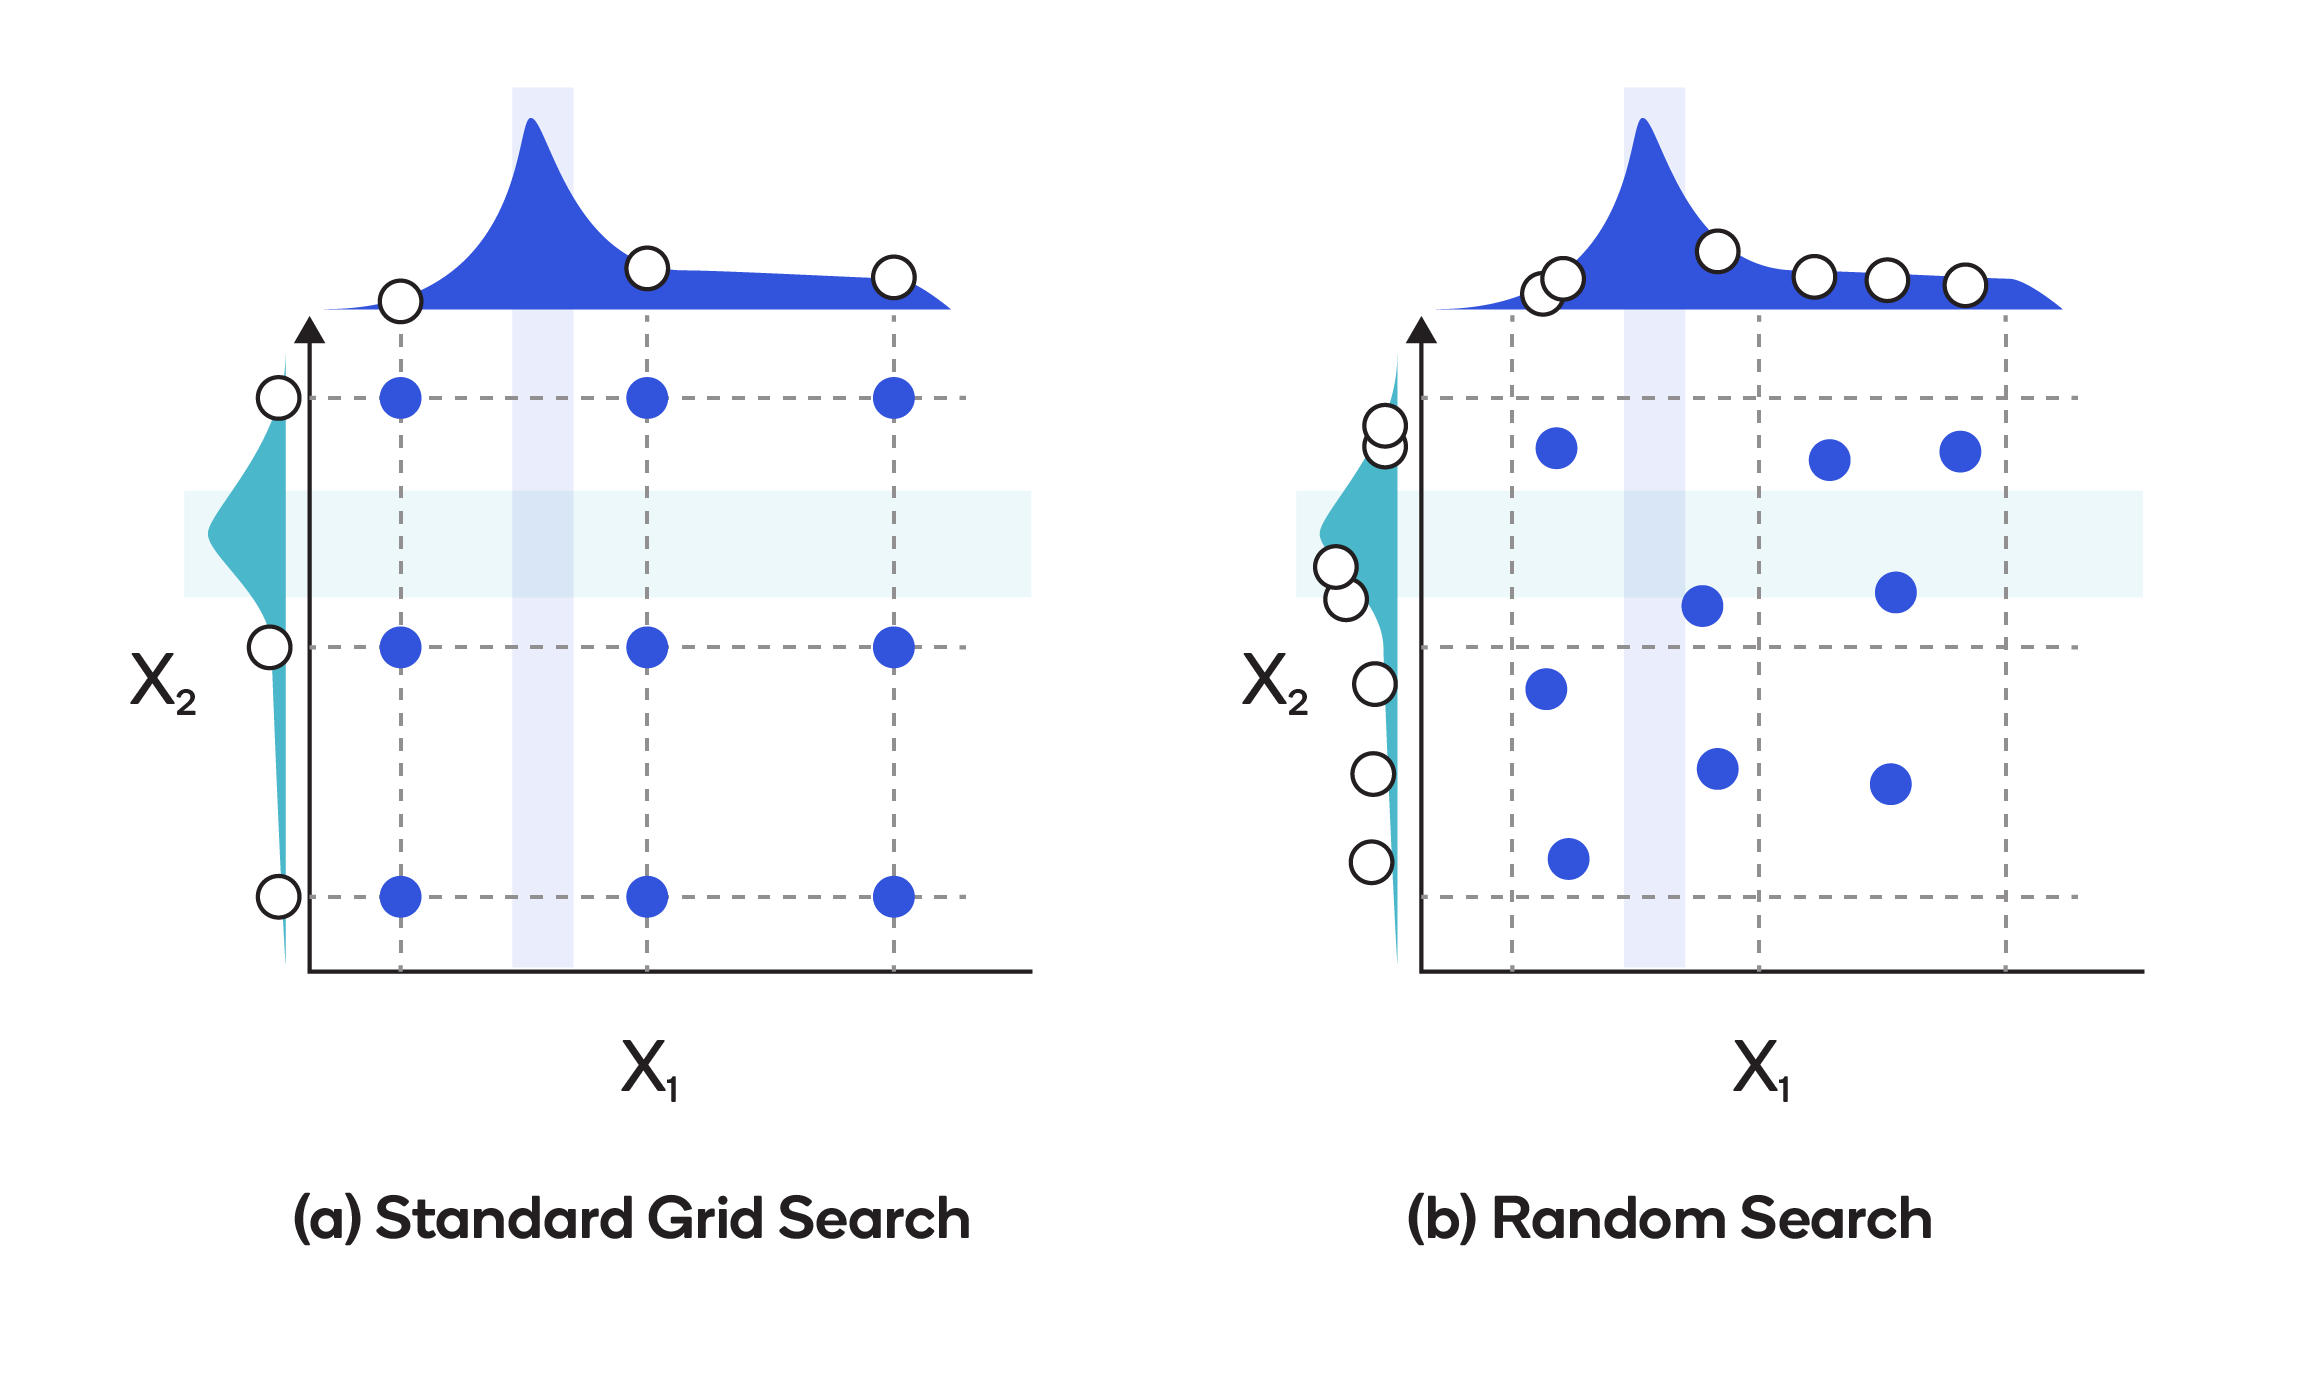
\includegraphics[width=\linewidth]{contents/chapter_3/resources/HyperParameter.png}
    \caption{Exemple de grille de recherche d’hyperparamètres. L’influence de chaque paramètre est ainsi mesurée au travers de cette grille, avec h1 et h2 deux hyperparamètres.}
    \label{fig:chapter_3:HyperParameter}
\end{figure}

Malheureusement, la modification de ces paramètres et le choix des meilleurs d’entre eux, conduit à un phénomène de surestimation des performances du modèle généré par une « procédure de comparaison multiple » [30], si nous n’employons pas certaines précautions. De plus, cet ajustement peut conduire à des situations de sur-apprentissage, les paramètres tentant de corréler au mieux aux données disponibles. Il est donc nécessaire de procéder à une évaluation rigoureuse des performances du modèle choisi, c’est-à-dire en restant objectif vis-à-vis de l’observation réalisée (ne pas procéder à des réglages supplémentaires à parti de cette étape). Différentes approches existent, avec pour la simple une validation croisée dans un schéma de type « holdout » (Figure 43), et pout la plus fonctionnel un schéma imbriqué de validation croisée pour la sélection des hyperparamètres et l’estimation du modèle.
  
\begin{figure}[H]
    \centering
    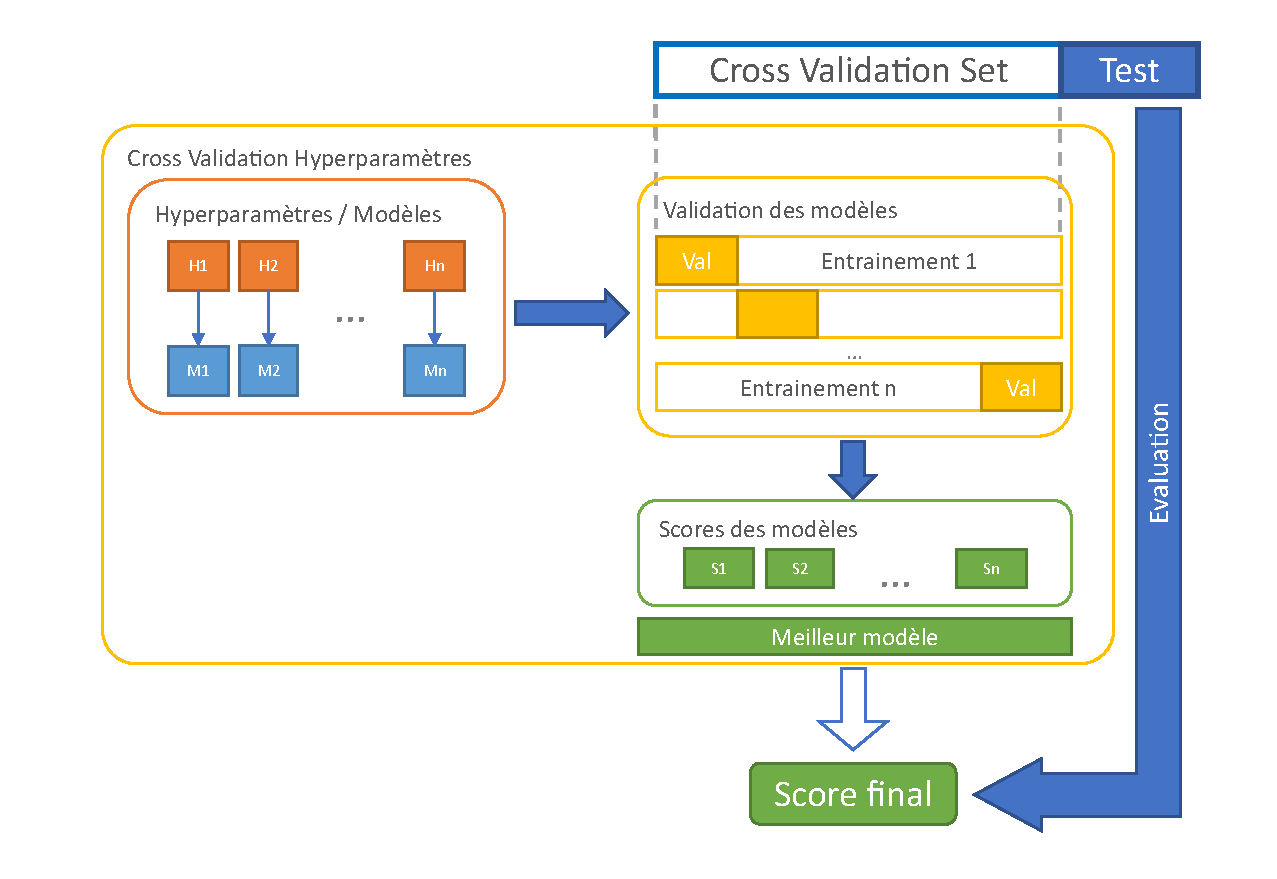
\includegraphics[width=\linewidth]{contents/chapter_3/resources/HyperParameterProcess.pdf}
    \caption{Modèle de validation type pour la sélection d’hyperparamètre.}
    \label{fig:chapter_3:HyperParameterProcess}
\end{figure}

\subsubsection{Fusion d’informations}
Dernier aspect de notre sujet, la fusion d’informations se définie comme l’action de « combiner des informations issues de plusieurs sources afin d’améliorer la prise de décision » [31]. De manière plus large, le groupe de travail européen FUSION tend à la décrire comme « le regroupement des informations issues de plusieurs sources et exploiter l’information regroupée afin de répondre à des questions, prendre des décisions, … ».
 
Figure 45 : Deux modes génériques de fusion. A gauche, l’utilisation de diverses sources permet une meilleure estimation finale. A droite, dans le cadre d’automates essentiellement, elle permet de réaffiner au plus juste un modèle de prédiction théorique.


Dimensionality reduction can be achieved in the following ways

	Feature Elimination: You reduce the feature space by eliminating features. This has a disadvantage though, as you gain no information from those features that you have dropped.

	Feature Selection: You apply some statistical tests in order to rank them according to their importance and then select a subset of features for your work. This again suffers from information loss and is less stable as different test gives different importance score to features. You can check more on this here.

	Feature Extraction: You create new independent features, where each new independent feature is a combination of each of the old independent features. These techniques can further be divided into linear and non-linear dimensionality reduction techniques.

Incertitude :
« L’incertitude est relative à la vérité d’une information, et caractérise son degré de conformité à la réalité. Elle fait référence à la nature de l’objet ou du fait concerné, à sa qualité, à son essence ou à son occurrence. »
Imprécision :
« L’imprécision concerne le contenu de l’information et mesure donc un défaut quantitatif de connaissance, sur une mesure. Elle concerne le manque d’exactitude en quantité, en taille, en durée, le manque de définition d’une proposition qui est ouverte à diverses interprétations ou qui a des frontières vagues et mal définies. »
Incomplétude : 
« L’incomplétude caractérise l’absence d’information apportée par la source sur certains aspects du problème. L’incomplétude des informations issues de chaque source est la raison principale qui motive la fusion. L’information fournie par chaque source est en général partielle, elle ne fournit qu’une vision du monde ou du phénomène observé, en ne mettant en évidence que certaines caractéristiques. »
Ambiguïté :
« L’ambiguïté exprime la capacité d’une information de conduire à deux interprétations. Elle peut provenir des imperfections précédentes, par exemple de l’imprécision d’une mesure qui ne permet pas de différencier deux situations, ou de l’incomplétude qui conduit à des confusions possibles entre les objets et des situations qui ne peuvent être séparées selon les caractéristiques mises en évidence par la source. Un des objectifs de la fusions est de lever les ambiguïtés d’une source grâce aux informations apportées par les autres sources ou par les connaissances supplémentaires. »
Conflit :
« Le conflit caractérise deux ou plusieurs informations conduisant à des interprétations contradictoires et donc incompatibles. Les situations conflictuelles sont fréquentes dans les problèmes de fusion, et posent toujours des problèmes difficiles à résoudre. »
Redondance :
« La redondance est la qualité des sources qui apportent plusieurs fois la même information. La redondance entre les sources est souvent observée, dans la mesure où les sources donnent des informations sur le même phénomène. Idéalement, la redondance est exploitée pour réduire les incertitudes et les imprécisions. »
Complémentarité :
« La complémentarité est la propriété des sources qui apportent des informations sur des grandeurs différentes. Elle vient du fait qu’elles ne donnent en général pas d’informations sur les mêmes caractéristiques du phénomène observé. Elle est exploitée directement dans le processus de fusion pour avoir une information globale plus complète et pour lever des ambiguïtés. »
Diversité : (due to multimodality) is the property that allows to enhance the uses, benefits and insights (such as those discussed in Section II), in a way that cannot be achieved with a single modality.[32]
Data fusion : is the analysis of several data sets such that different data sets can interact and inform each other.[32]

Trouble using fusion : The McGurk effect serves as an indication that in real-life scenarios, data fusion can take paths much more intricate than simple summation of information. Not less important, it serves as a lesson that fusing modalities can yield undesired results and severe degradation of performance if the underlying relationships between modalities are not properly understood. [32]s

Problème syllabes -> « ba » « ga » devient « na »
